\chapter{Validación y verificación}
\label{cap:capitulo6}

\begin{quote}
	\begin{flushright}
		\small ``\textit{Pon el programa a funcionar, y que Dios nos pille confesados.}'' \\
		--- Profesor Salvador Villena Morales (2013).
	\end{flushright}
\end{quote}

\vspace{8em}

Como fase final de cualquier proyecto, una vez terminada la implementación, es el momento de ejecutar las pruebas de validación sobre el sistema desarrollado.

En primer lugar debemos \textbf{verificar} que el proyecto cumple los requisitos propuestos. Otro paso importante será comprobar que el sistema es \textbf{válido} para solucionar nuestro problema, donde entran componentes relacionados con el rendimiento.

\newpage

\section{Servicio de reproducción}

El servicio de reproducción es el \textbf{demonio} desarrollado para reproducir las partituras y despachar peticiones del \textit{socket} y del mando (a través del \acrshort{UART}). Ya que funcionará en segundo plano será muy importante que la implementación controle adecuadamente todos los errores posibles para evitar cierres inesperados.

Algunos de los problemas más comunes son los \textbf{errores de memoria}, sobre todo en un lenguaje que no la gestiona automáticamente. Para validar la gestión de memoria, hemos utilizado la herramienta \textbf{Valgrind}, que nos muestra todos los posibles errores relativos a memoria, tales como:

\begin{itemize}
	\item Acceder a una dirección ilegal.
	\item No liberar la memoria reservada.
\end{itemize}

Esta aplicación no funciona correctamente en \textit{Raspbian}, por tanto hicimos la prueba en un sistema con \textbf{\textit{Ubuntu}}. La gestión de memoria es similar, aunque difieren algunas longitudes de variables, sin embargo, eso lo gestiona el \textbf{compilador} y no depende de la programación.

Solo hubo un módulo que no se pudo comprobar: la salida \acrshort{GPIO}, ya que es dependiente de la plataforma \textit{hardware}. A pesar de ello, solo hace una llamada a \code{mmap()} al inicio y otra a \code{munmap()} al final, de forma que los errores serían visibles nada más arrancar el programa.

\subsection{Requisitos}

Para validar los distintos módulos se realizó una \textbf{batería de pruebas} sobre ellos, respectivas a la entrada de datos que esperan, y estudiamos la salida para verificar que coincide con lo requerido.

\subsubsection{Entrada de archivos MIDI}

El principal requisito del analizador de \acrshort{MIDI} es que debe aceptar cualquier fichero de formato válido, no solo aquellos adaptados a nuestro proyecto. Hemos analizado hasta \textbf{46 archivos} \acrshort{MIDI} de diferentes orígenes:

\begin{enumerate}
	\item 42 piezas estándar, con varias pistas y diferentes instrumentos ---incluyendo batería---.
	\item 4 de formato específico, con 2 a 4 pistas.
\end{enumerate}

De acuerdo a lo especificado, el \textit{software} analiza correctamente archivos \acrshort{MIDI} con varias \textbf{pistas simultáneas}, y de cualquier \textbf{división de tiempo}, en formato $ticks / \quarternote$, descartando los \textbf{eventos específicos} del sistema.

\subsubsection{Planificador y control}

El planificador debe ser capaz de atender ágilmente cualquier archivo \acrshort{MIDI} con varias pistas. Para probarlo, utilizamos el \textbf{simulador} de reproducción, construido para este propósito (véase la sección \ref{subsec:simulador_reproduccion}). Esta aplicación fue muy útil para pulir cualquier detalle de programación, y probó que el \textbf{diseño} del algoritmo de planificación es correcto desde el primer momento.

El concepto de la \textbf{interfaz de salida} también fue comprobado, a pesar de que la verificación de la implementación requiere la \acrshort{PCB}, de la que dispondremos más adelante.

Por otro lado, la aplicación del \textbf{terminal} nos sirvió para dos cosas:

\begin{enumerate}
	\item Verificar el \textbf{protocolo} de comunicación.
	\item Validar la gestión \textbf{concurrente} entre la hebra de reproducción y la del \textit{socket}.
\end{enumerate}

En base a las pruebas realizadas, el funcionamiento coincide con lo esperado, y controla adecuadamente los siguientes problemas en la entrada:

\begin{enumerate}
	\item Sin argumentos.
	\item Parámetros incorrectos.
	\item Argumentos muy largos, con un nombre de archivo ficticio de 40 \textit{KiB} (el \textit{buffer} está limitado a 4 \textit{KiB}).
\end{enumerate}

\subsubsection{Mando y metrónomo}

La validación de esta parte del sistema requería disponer de la \acrshort{PCB}, pero tenía una complejidad considerable y era necesario realizar incluso prototipos de \textit{software} para el \acrshort{UART}.

La solución a este problema fue utilizar un \textbf{\textit{Arduino}} para simular el mando a distancia, y un \acrshort{led} para comprobar el funcionamiento del metrónomo. Esto supuso una serie de cuestiones:

\begin{enumerate}
	\item \textit{Arduino} funciona a 5 \textit{V}, mientras que \textit{Raspberry Pi} trabaja a 3,3 \textit{V}.
	\item La corriente del \acrshort{GPIO} del \textit{Raspberry Pi} está limitado a 50 \textit{mA}, a cargo del usuario.
\end{enumerate}

La solución a estos problemas fue \textbf{diseñar} un pequeño circuito electrónico con un \textbf{divisor de tensión} y una resistencia para el \acrshort{led}.

\smallskip

\begin{figure}[H]
	\noindent \begin{centering}
		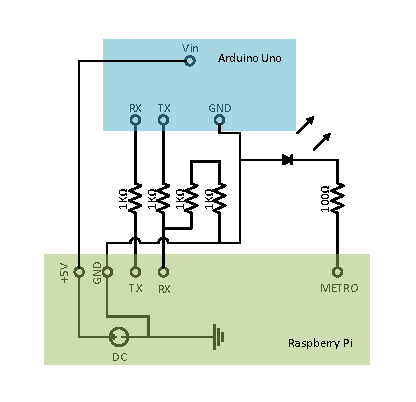
\includegraphics[width=\linewidth/2]{capitulo6/proto_esquema}
		\par\end{centering}
	\smallskip
	\caption{\label{fig:proto_esquema} Esquema de la placa de prueba.}
\end{figure} 

\smallskip

De acuerdo a la fórmula de un divisor de tensión resistivo \cite{wiki_divtension}, a la salida en el pin RX de \textit{Raspberry Pi} tendremos:


\begin{equation}
	V_{out} = V_{in} \times \frac{R_2}{R_1 + R_2} = 5 \; V \times \frac{2 \; K\Omega}{3 \; K\Omega} = 3,\stackrel{\frown}{3} \; V
\end{equation}


Por otro lado, con la resistencia junto al \acrshort{led}, la corriente está muy por debajo del límite de 50 \textit{mA}, según la \textbf{ley de Ohm} \cite{wiki_ohm}:

\begin{equation}
	I = \frac{V}{R} = \frac{3.3 \; V}{100 \; \Omega} = 33 \; mA
\end{equation}

El resultado fue el siguiente: \textit{Raspberry Pi} alimenta a Arduino, y se comunica mediante el \acrshort{UART} con un circuito de seguridad para asegurar el voltaje de la señal. Además, tenemos un indicador luminoso para verificar el metrónomo.

Por simplicidad, programamos una batería de pruebas para que Arduino suplantara al mando generando distintas cadenas aleatorias, variando los siguientes parámetros:

\begin{enumerate}
	\item Número de serie del mando.
	\item Botones pulsados.
	\item Señal de batería baja.
	\item Longitud de la cadena (generar errores).
\end{enumerate}

El despachador de \acrshort{UART} del servicio atiende correctamente las señales transmitidas. Si el nº de serie no coincide con el registrado o recibe un aviso de batería baja, \textbf{emite un mensaje en el \textit{log}} del sistema y descarta el resto del mensaje.

Si eventualmente llegan menos \textit{bytes} de los 10 previstos, el programa sigue esperando el resto (otra pulsación), entonces detecta una \textbf{corrupción} de datos y vacía el \textit{buffer}. Es importante tener este improbable supuesto en cuenta para no bloquear indefinidamente el receptor.

\smallskip

\begin{figure}[H]
	\noindent \begin{centering}
		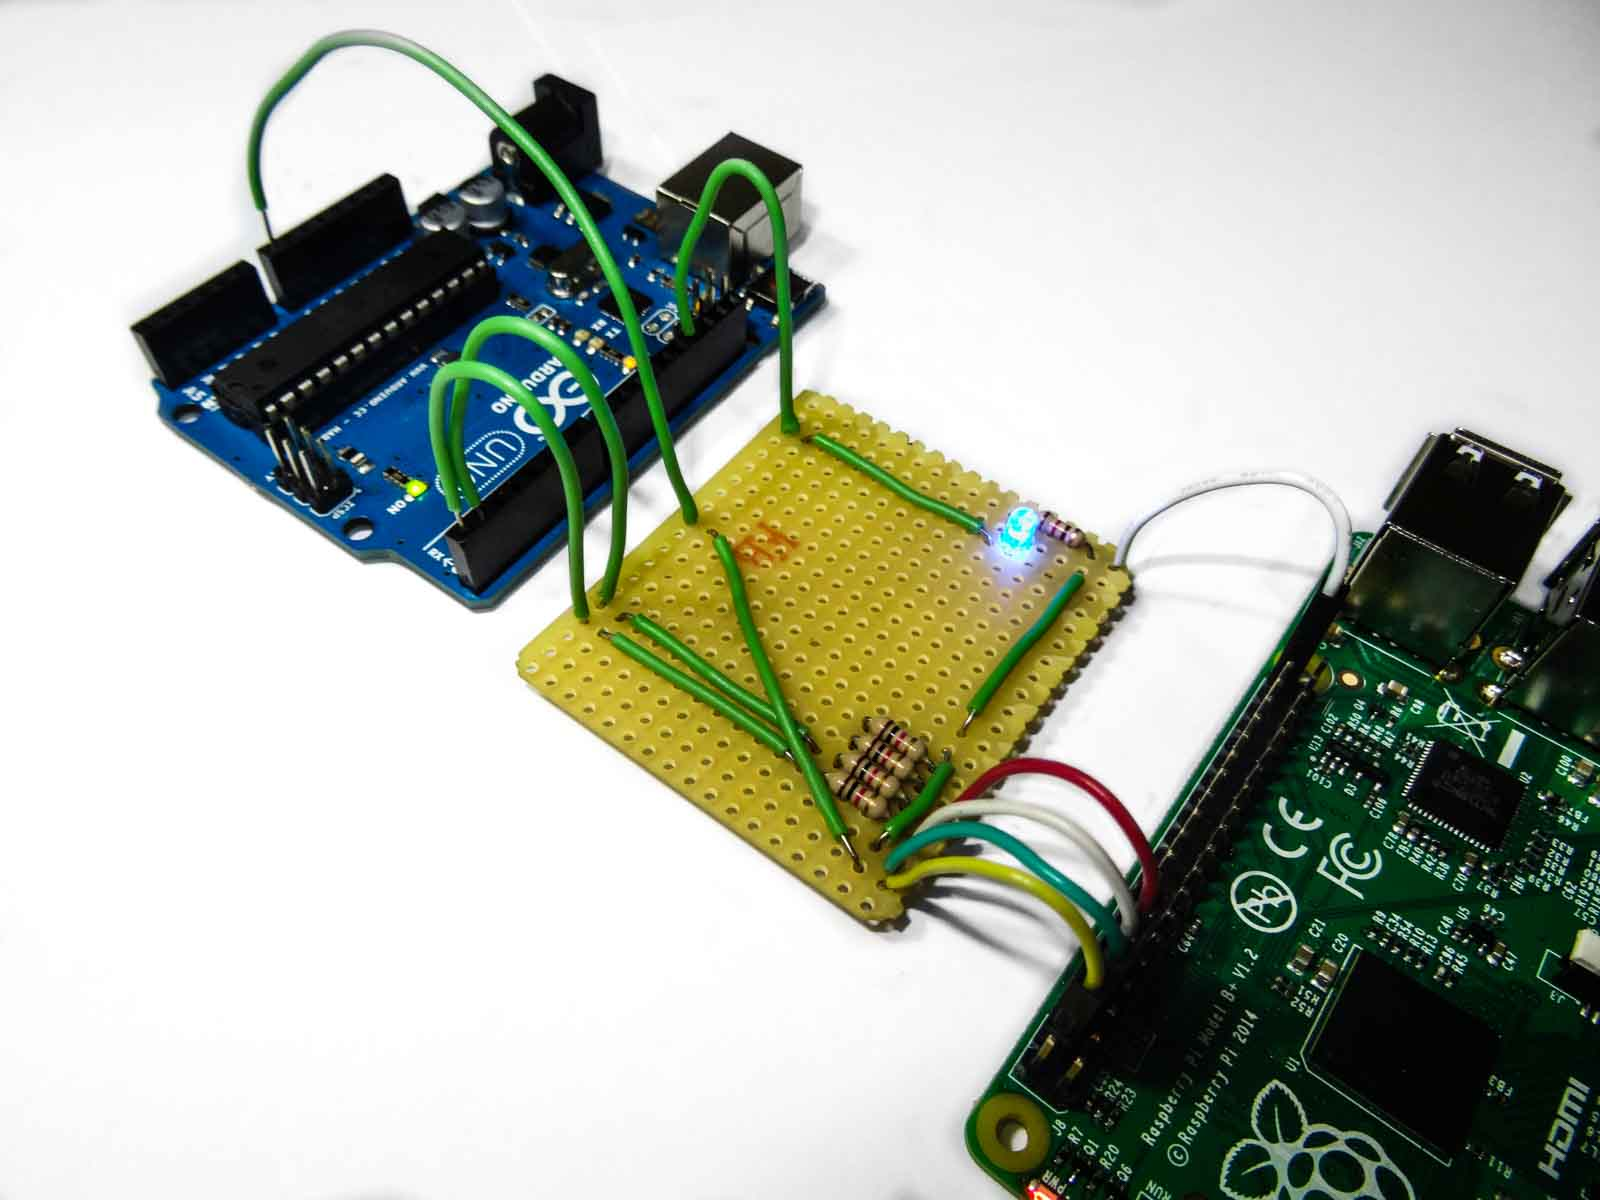
\includegraphics[width=\linewidth*3/4]{capitulo6/proto_uart}
		\par\end{centering}
	\smallskip
	\caption{\label{fig:proto_uart} Placa de prueba entre Arduino y Raspberry Pi.}
\end{figure} 

\smallskip

\subsubsection{Funcionamiento continuado}

Es importante comprobar que el demonio es estable y se mantiene activo durante un tiempo considerable. Para ello, hemos dejado el sistema reproduciendo una lista repetidamente durante casi 40 horas, manteniendo el funcionamiento y el uso de memoria.

A continuación, mostramos una captura de pantalla de la aplicación \code{top}, que detalla el \textbf{uso de recursos} del servicio en segundo plano:

\smallskip

\begin{figure}[H]
	\noindent \begin{centering}
		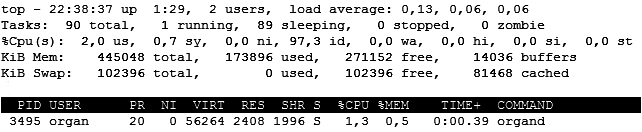
\includegraphics[width=\linewidth*3/4]{capitulo6/cap_top}
		\par\end{centering}
	\smallskip
	\caption{\label{fig:cap_top} Uso de recursos del sistema.}
\end{figure} 

\smallskip

El programa muestra que el demonio en funcionamiento consume un \textbf{1,3\% de \acrshort{CPU}} y \textbf{5,27 \textit{MiB} de memoria} RAM, entre privada y compartida.

\subsection{Rendimiento}

En las líneas siguientes estudiaremos la eficiencia de los módulos más importantes del sistema, a través de distintos procedimientos.

Para cronometrar el tiempo utilizaremos la función \code{clock\_gettime()} de la \textbf{biblioteca de tiempo-real} de \acrshort{POSIX}. Emplearemos el \textbf{reloj monotónico} del sistema, que tiene una resolución del orden de 1 \textit{ns}.

\subsubsection{Analizador MIDI}

En primer lugar, vamos a medir el tiempo que tarda el módulo \acrshort{MIDI} en analizar un archivo completo. Para ello, insertamos en la función \code{midi\_init()} el código necesario para cronometrar, según hemos descrito anteriormente.

Hemos medido 5 veces el tiempo de análisis de \textbf{10 partituras}, con el siguiente resultado:

\smallskip

\begin{figure}[H]
	\noindent \begin{centering}
		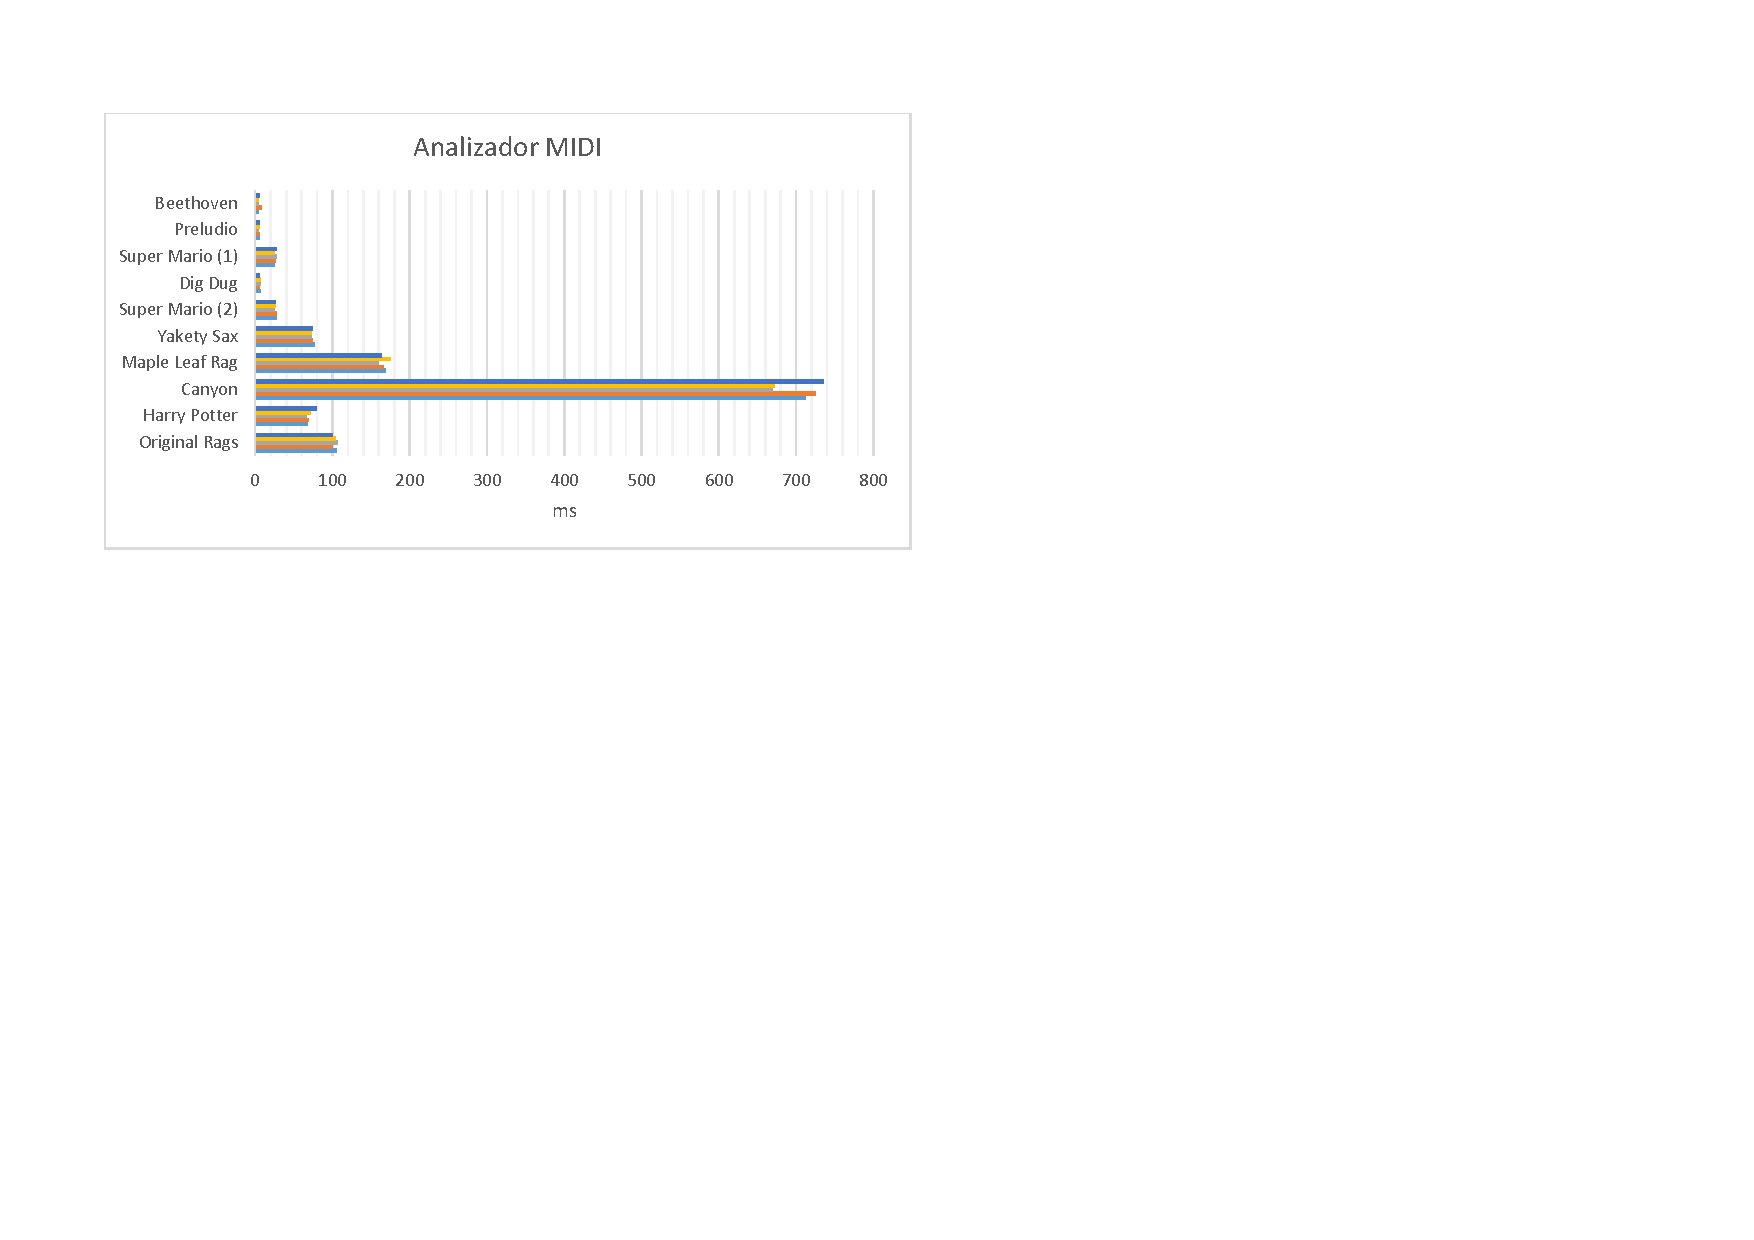
\includegraphics[width=\linewidth*3/4]{capitulo6/lat_midi}
		\par\end{centering}
	\smallskip
	\caption{\label{fig:lat_midi} Tiempo de ejecución del analizador MIDI.}
\end{figure} 

\smallskip

Podemos comprobar que el tiempo de análisis es bastante aceptable, manteniendo tiempos del orden de 100 \textit{ms}. Las cuatro primeras partituras son de \textbf{creación propia}, el peor caso es ``Super Mario (1)'', que tarda 27 \textit{ms}. La \textbf{ejecución más veloz} ha sido la de ``Beethoven'', con 4,62 \textit{ms}.

El resto de piezas forman parte de la batería de pruebas y no se utilizarán finalmente. El archivo ``Canyon'' representa un \textbf{valor atípico} con un tiempo de 700 \textit{ms}. Se trata de una antigua demostración de \acrshort{MIDI} para \textit{Windows 98}, contiene 7 pistas y una serie de \textbf{complejas instrucciones} que no utilizaremos en un funcionamiento normal.

\smallskip

\begin{figure}[H]
	\noindent \begin{centering}
		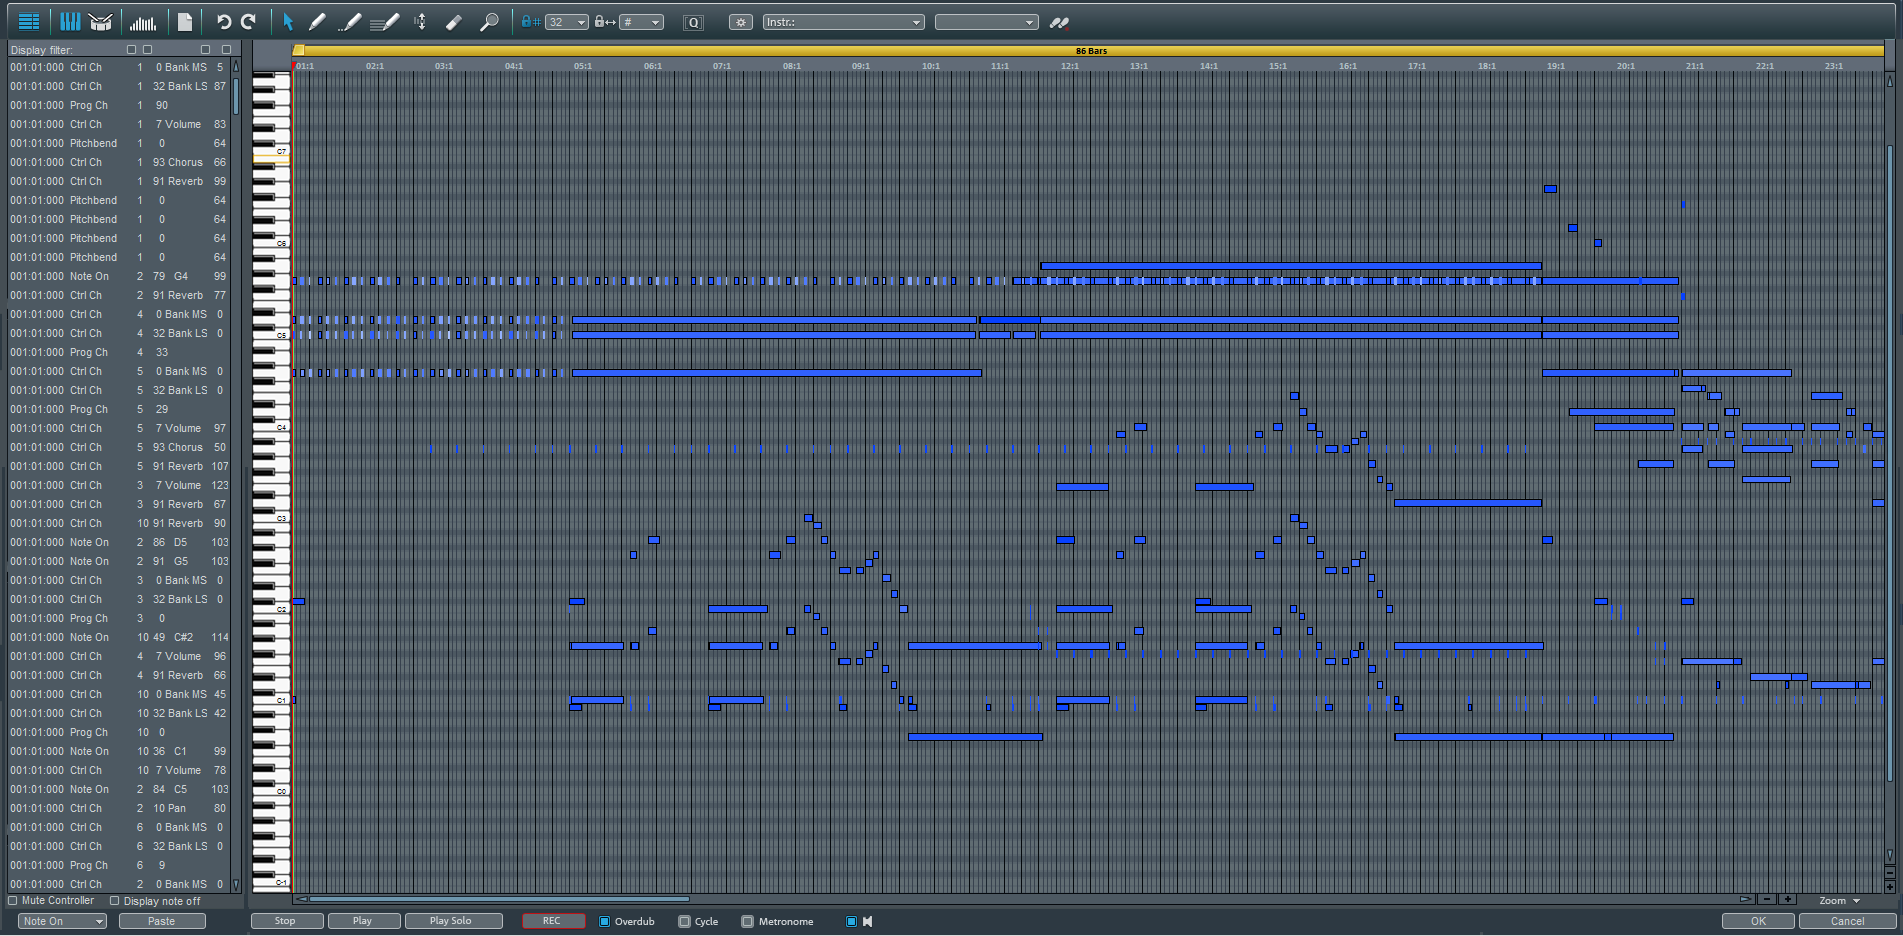
\includegraphics[width=\linewidth*3/4]{capitulo6/cap_canyon}
		\par\end{centering}
	\smallskip
	\caption{\label{fig:cap_canyon} Edición de canyon.mid con Magix Music Maker 2015.}
\end{figure} 

\smallskip

\subsubsection{Planificador}

Para analizar el rendimiento del planificador, medimos el \textbf{tiempo de cada iteración} del bucle principal. Para obtener los datos más adecuados al funcionamiento real, utilizaremos dos partituras específicas: la \textit{Oda a la Alegría} de Beethoven y el \textit{Preludio nº 4} de Bach:

\smallskip

\begin{figure}[H]
	\noindent \begin{centering}
		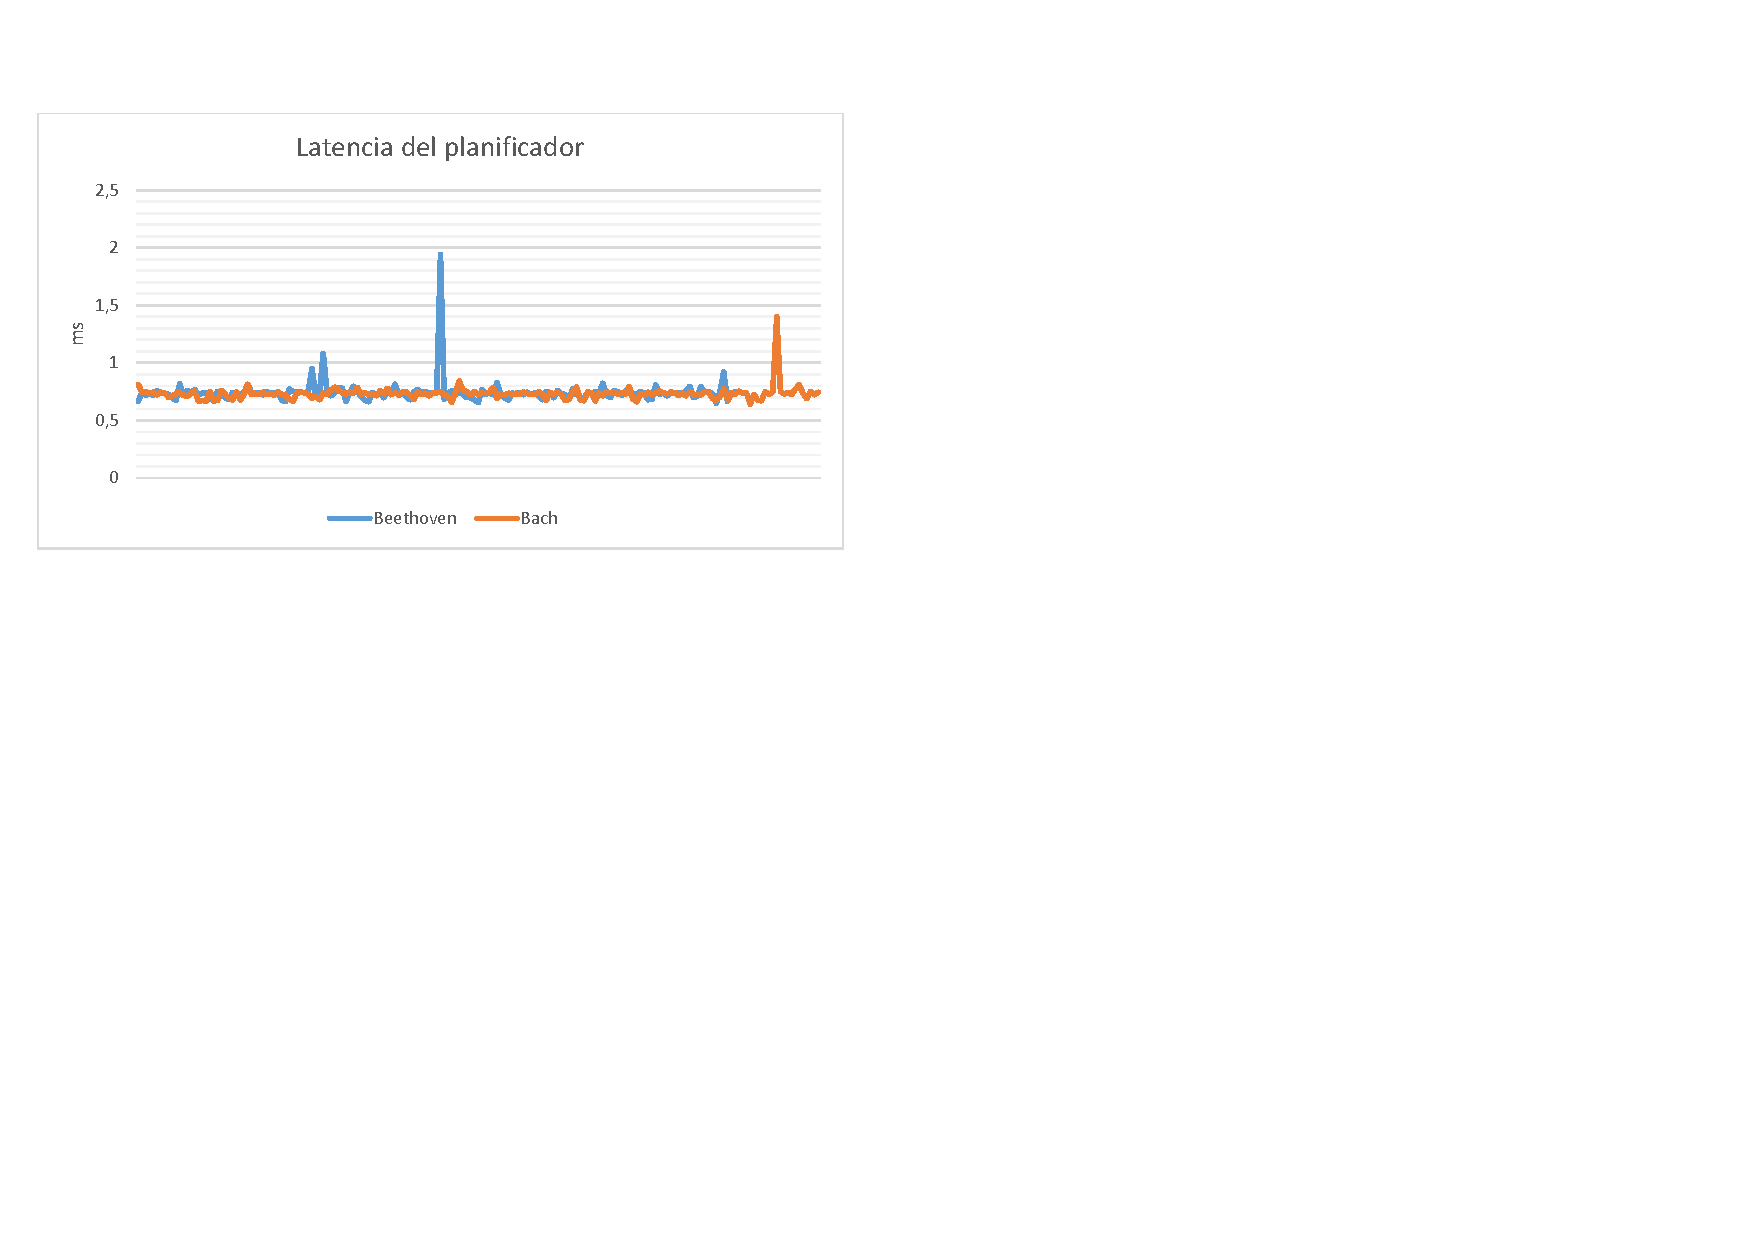
\includegraphics[width=\linewidth*3/4]{capitulo6/lat_sched}
		\par\end{centering}
	\smallskip
	\caption{\label{fig:lat_sched} Tiempo de ejecución del planificador.}
\end{figure} 

\smallskip

Los datos indican que el \textbf{ciclo medio} tarda $738 \; \mu s$. Ya que el algoritmo está diseñado para avanzar tantos eventos como pueda dentro de cada pista, era previsible encontrar tiempos \textbf{ligeramente superiores} en algunos casos. Aún así, el peor tiempo es de 1,94 \textit{ms}, un lapso imperceptible por el usuario.

\subsubsection{Salida GPIO}

Es ahora el momento de medir el tiempo que tarda el programa en enviar los datos a la \acrshort{PCB} a través del \acrshort{GPIO}. En este caso, vamos a contrastar los datos de dos implementaciones:

\begin{enumerate}
	\item Volcado de notas del prototipo en Python.
	\item Función \code{output\_update()} de la implementación final en C.
\end{enumerate}

La siguiente imagen ilustra los datos obtenidos:

\smallskip

\begin{figure}[H]
	\noindent \begin{centering}
		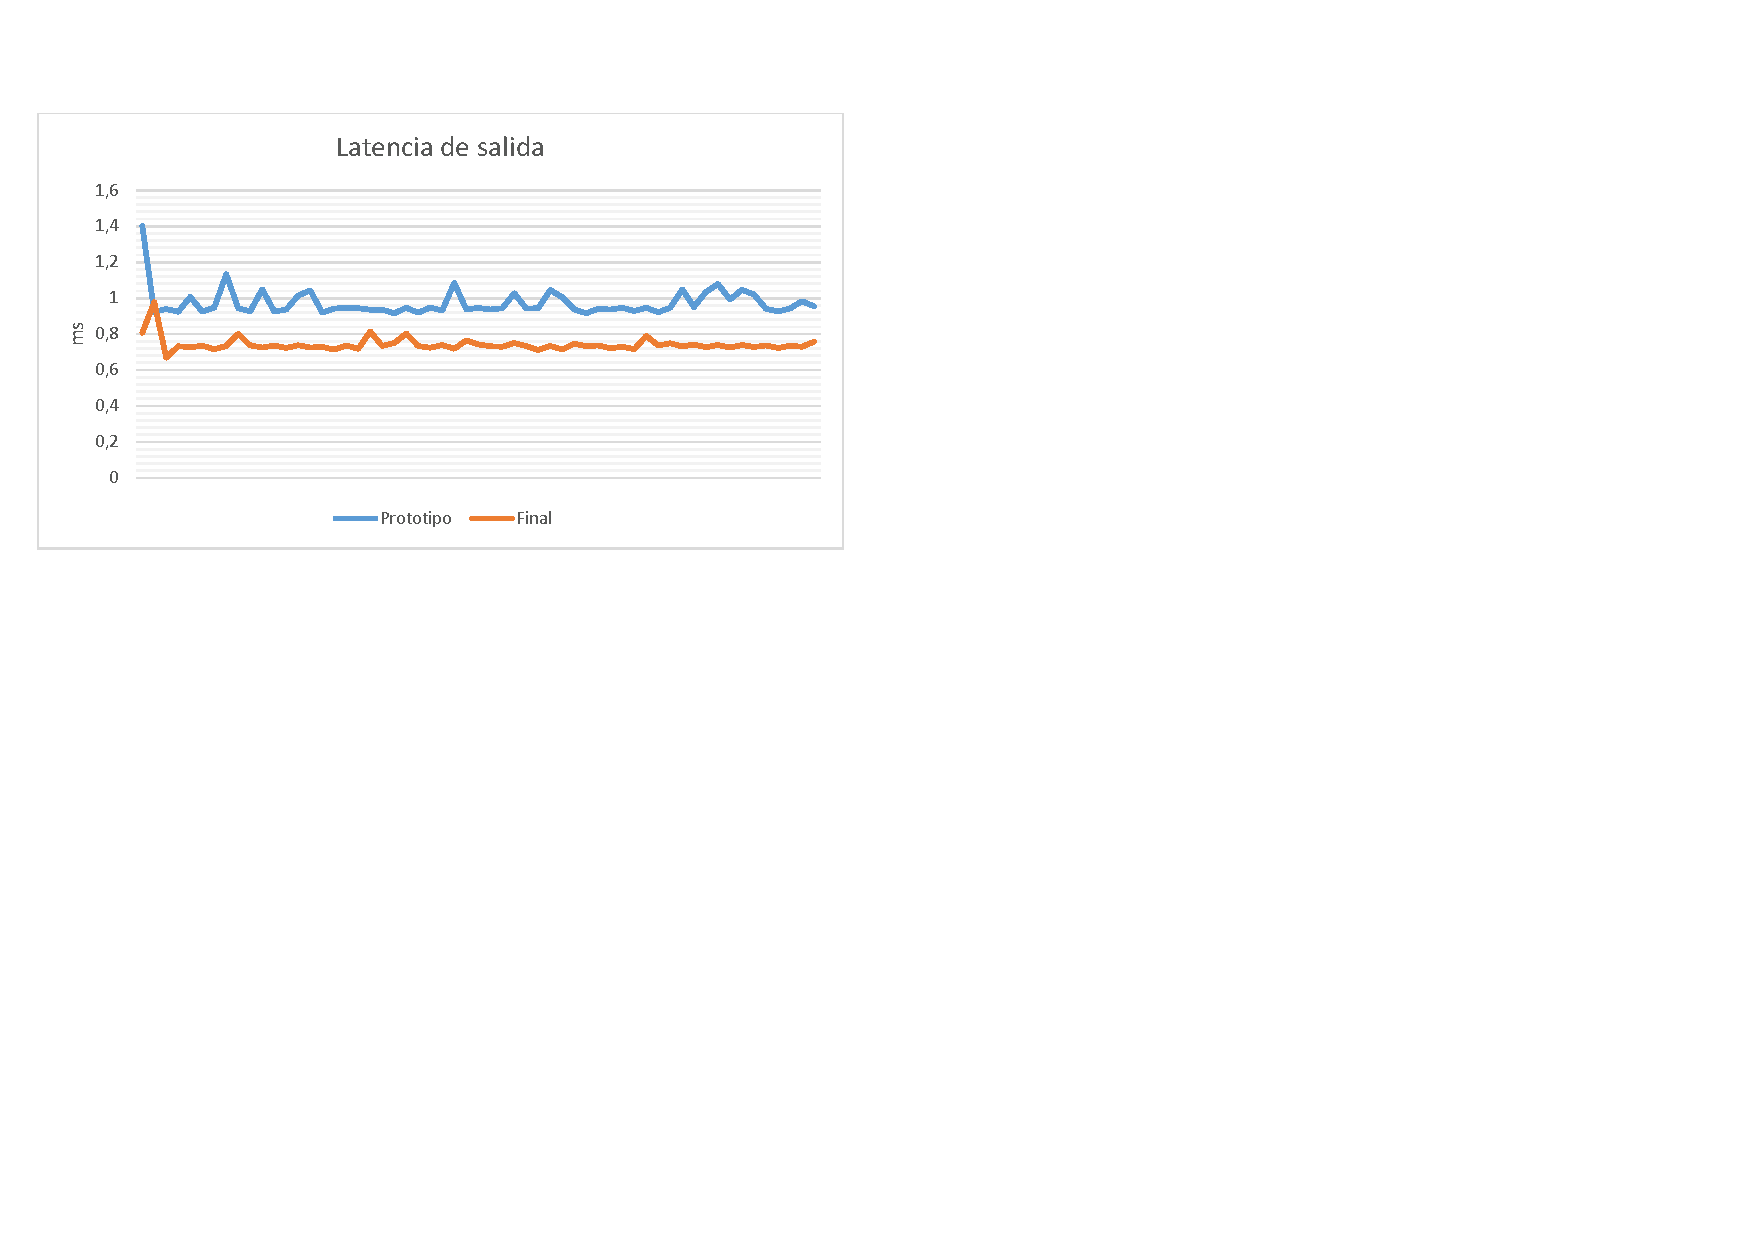
\includegraphics[width=\linewidth*3/4]{capitulo6/lat_gpio}
		\par\end{centering}
	\smallskip
	\caption{\label{fig:lat_gpio} Tiempo de ejecución de la salida a GPIO.}
\end{figure}

\smallskip

Los datos más relevantes son los siguientes:

\smallskip

\begin{table}[H]
	\begin{center}
		\begin{tabular}{|l|r|r|}
			\hline & \textbf{Prototipo} & \textbf{Final} \\ 
			\hline \textbf{Peor caso} & $1401 \; \mu s$ & $977 \; \mu s$ \\
			\hline \textbf{Media} & $973 \; \mu s$ & $738 \; \mu s$ \\
			\hline
		\end{tabular}
		\smallskip
		\caption{\label{tab:lat_gpio} Latencia de la salida al GPIO.}
	\end{center}
\end{table}

\smallskip

El hecho de que el peor caso esté claramente en las \textbf{primeras llamadas} a la función se explica por la implementación del acceso al \acrshort{GPIO} como un \textbf{periférico mapeado} en memoria. Inicialmente el acceso es notablemente superior, hasta que la \textbf{memoria caché} almacena la dirección, acelerando los accesos posteriores.

A pesar de que Python es un lenguaje \textbf{interpretado}, la biblioteca para acceder al \acrshort{GPIO} está implementada en C, lo que nos proporciona un buen \textbf{rendimiento}.

\newpage

\section{Interfaz web}

La interfaz principal está implementada como un servicio \textit{web} sito en el propio \textit{Raspberry Pi}. Como cualquier servidor estándar, escucha el \textbf{puerto 80} del protocolo \acrshort{TCP} a través de la interfaz de red.

Uno de los pasos previos a las pruebas de validación es configurar el módulo \acrshort{PHP} en \textbf{modo \textit{development}} (desarrollo), para recibir información y alertas que nos permitirán detectar errores eficazmente.

\subsection{Red de área local}

El sistema no está ideado para ser utilizado desde Internet, pero sí en una red de área local sencilla, bien a través de cable o bien conectando un adaptador WiFi por \acrshort{USB}.

Sin embargo, nuestro \textit{Raspberry Pi} va a estar \textbf{conectado a Internet} durante la fase de desarrollo, tanto para descargar los paquetes necesarios y recibir actualizaciones como para facilitar la verificación. Conectaremos el dispositivo a nuestro \textit{router} mediante un cable \textit{Ethernet} directo.

Para \textbf{recibir conexiones} \acrshort{HTTP} desde Internet, es necesario configurar el router y \textbf{desviar el puerto \acrshort{TCP} 80} hacia la dirección \acrshort{IP} que hayamos asignado al \textit{Raspberry Pi}. 

En lugar de hacer esto, vamos a crear una \textbf{segunda red local} a la que dirigiremos todos los puertos de entrada, convirtiéndola en una \textbf{zona desmilitarizada} (\acrshort{DMZ}, \textit{\acrlong{DMZ}}). La \textbf{red doméstica} quedará al otro lado del \textit{firewall} del \textit{router}.

\smallskip

\begin{figure}[H]
	\noindent \begin{centering}
		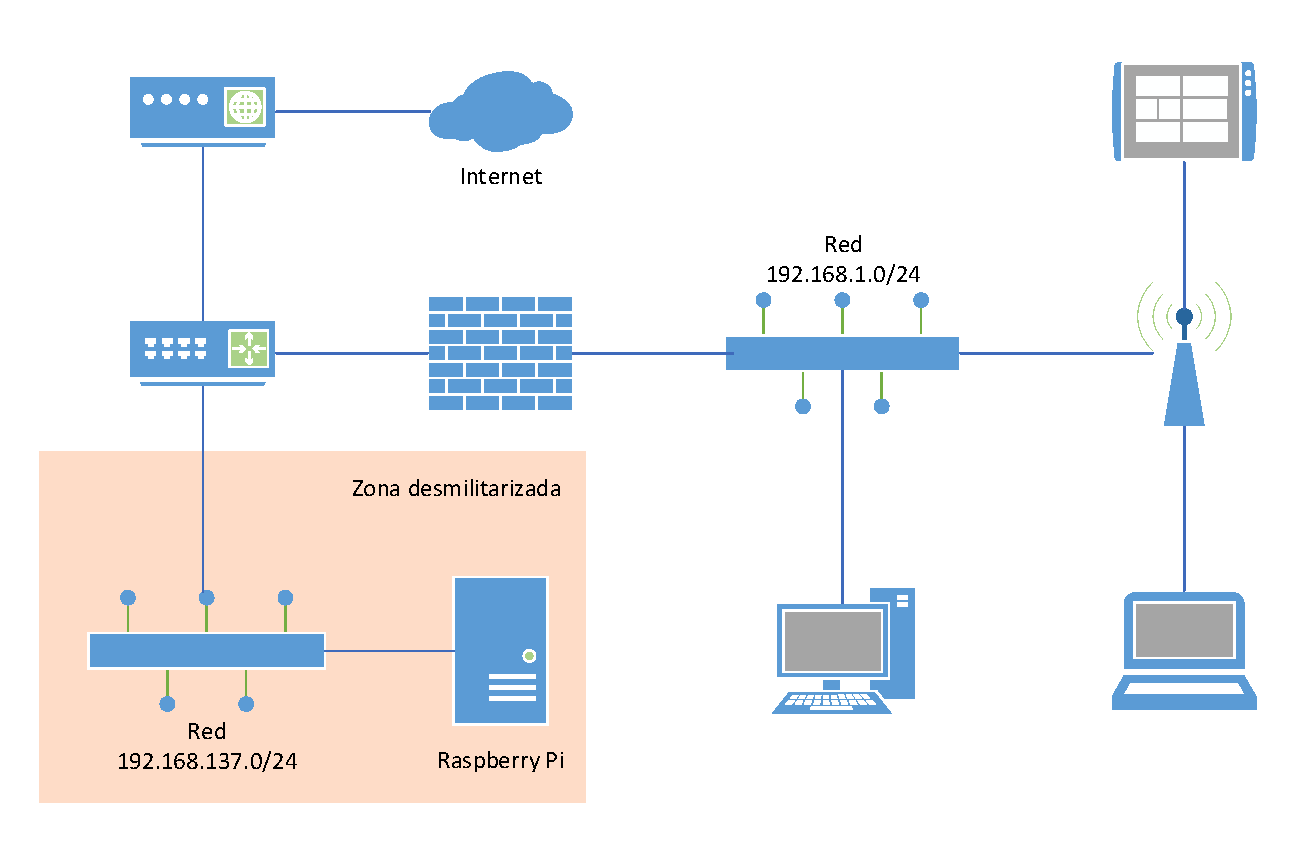
\includegraphics[width=\linewidth*3/4]{capitulo6/network}
		\par\end{centering}
	\smallskip
	\caption{\label{fig:network} Diagrama de red conectada al Raspberry Pi.}
\end{figure}

\smallskip

\subsection{Requisitos}

Ya que ésta es una aplicación de usuario, desplegaremos las pruebas típicas de entradas de datos en formularios. Una regla importante de la \textbf{programación defensiva} es no permitir al usuario utilizar incorrectamente el sistema.

\bigskip

\begin{quote}
	\small \flushright ``\textit{Haced los programas como si el usuario tratara el teclado a patadas.}'' \\
	--- Profesor Joaquín Fernández Valdivia (2009).
\end{quote}

\bigskip

Además, podremos conectarnos desde \textbf{varios clientes} para comprobar que el sistema responde correctamente ante peticiones simultáneas.

\subsubsection{Vista y controlador}

La implementación de las interfaces de entrada y salida sigue este principio:

\begin{itemize}
	\item Si un error proviene del \textbf{usuario}, se comporta asertivamente (muestra un error).
	\item Si procede de un \textbf{error interno}, actúa pasivamente o muestra un error genérico.
\end{itemize}

Hemos contemplado los siguientes supuestos:

\begin{description}
	\item[Errores externos] Producidos por el usuario. Se muestra un error.
	
	\begin{enumerate}
		\item Se intenta poner un nombre nulo a una lista o una obra.
		\item Se consulta por \acrshort{URL} una lista que no existe.
		\item Se llama al controlador sin un argumento válido.
	\end{enumerate}
	
	\item[Errores internos] Se pueden producir por una incoherencia entre la interfaz y el demonio. La interfaz los intenta recuperar.
	
	\begin{enumerate}
		\item Si desde un terminal se ejecuta la reproducción de una pieza que \textbf{no está registrada} en la base de datos, se muestra el nombre del archivo y se oculta la lista de reproducción.
		
		\item Si se \textbf{elimina} la pieza o la lista de reproducción en curso, el sistema se comporta como en el caso anterior. Cuando la pieza acaba y el servicio intenta cargar un archivo que no existe, pasa al siguiente. A pesar de que la reproducción se haga \textbf{en bucle}, si todos los archivos fallan, \textbf{el sistema se detiene} (de forma similar a pulsar \textit{Stop}).
	\end{enumerate}
\end{description}

\subsubsection{Formularios}

Como describimos en la sección \ref{subsec:web_seguridad} del capítulo de implementación, los formularios tienen una \textbf{doble capa} de seguridad:

\begin{enumerate}
	\item La \textbf{vista} en \acrshort{HTML} configura los campos para alertar al usuario si deja alguno en blanco o se excede del límite. El formulario \textbf{no se acepta} hasta que todas las entradas cumplan las condiciones.
	
	\item El \textbf{controlador} vuelve a comprobar las longitudes de cadena, filtra los mensajes para evitar inyección de código, y muestra un error si algún dato no está conforme.
\end{enumerate}

Realizaremos las siguientes pruebas en formularios:

\begin{enumerate}
	\item Dejar un campo \textbf{en blanco}. El navegador nos impide continuar.
	
	\smallskip
	
	\begin{figure}[H]
		\noindent \begin{centering}
			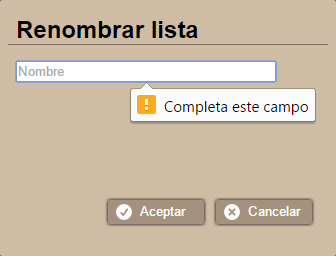
\includegraphics[width=\linewidth/3]{capitulo6/cap_camponulo}
			\par\end{centering}
		\smallskip
		\caption{\label{fig:cap_camponulo} Alerta al dejar un campo nulo.}
	\end{figure}
	
	\smallskip
	
	Sin embargo, es muy sencillo \textbf{eliminar la restricción} del formulario en el navegador:
	
	\smallskip
	
	\begin{figure}[H]
		\noindent \begin{centering}
			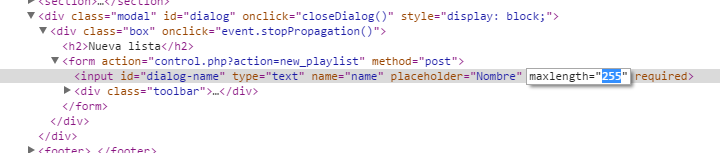
\includegraphics[width=\linewidth*3/4]{capitulo6/cap_hackform}
			\par\end{centering}
		\smallskip
		\caption{\label{fig:cap_hackform} Herramientas de desarrollo en Chrome.}
	\end{figure}
	
	\smallskip
	
	Al hacer esto, podemos dejar efectivamente el campo en blanco, pero entonces el \textbf{controlador} detectará este hecho y emitirá igualmente un error:
	
	\smallskip
	
	\begin{figure}[H]
		\noindent \begin{centering}
			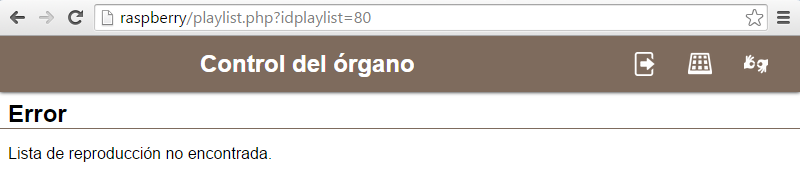
\includegraphics[width=\linewidth*3/4]{capitulo6/cap_error}
			\par\end{centering}
		\smallskip
		\caption{\label{fig:cap_error} Mensaje de error en la interfaz.}
	\end{figure}
	
	\smallskip
	
	\item Alcanzar el \textbf{límite} de tamaño permitido. La aplicación se comporta de la misma forma que en el caso anterior, a excepción de que, si \textbf{forzamos} la entrada de texto, el controlador \textbf{descartará} el texto más allá del límite especificado.
	
	\item \textbf{Inyectar código \acrshort{SQL}} en el formulario. El controlador filtra la cadena e introduce los \textbf{caracteres de escape} adecuados para evitar la inyección. La pieza o la lista quedan nombradas con el código tal como se escribe.
	
	\item Introducir una \textbf{contraseña incorrecta}. De acuerdo a lo descrito en la sección \ref{subsec:impl_portada} de implementación, el programa se bloquea 2 segundos y retorna con un aviso:
	
	\smallskip
	
	\begin{figure}[H]
		\noindent \begin{centering}
			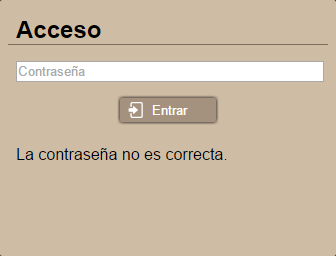
\includegraphics[width=\linewidth/3]{capitulo6/cap_errclave}
			\par\end{centering}
		\smallskip
		\caption{\label{fig:cap_errclave} Mensaje de error en la contraseña.}
	\end{figure}
	
	\smallskip
	
	\item Inyectar \textbf{código shell}. El controlador evita la inyección de la misma manera, escapando la cadena de entrada, y se intenta acceder al sistema con la cadena introducida como clave.
	
\end{enumerate}

\subsubsection{Carga de partituras}

Como interfaz de cara al usuario, la subida de partituras al servidor solo permite almacenar archivos \acrshort{MIDI} de hasta 1 \textit{MiB}. La batería de pruebas ha sido la siguiente:

\begin{enumerate}
	\item Subir una partitura válida. Se almacena sin mayor problema y aparece en la lista.
	\item Subir una partitura compuesta solo por \textbf{silencios} musicales. Se almacena y se muestra.
	\item Subir un archivo de \textbf{formato incorrecto} con extensión \code{.mid} de más de 1 \textit{MiB}. Aparece un error, explicando el tamaño como motivo.
	\item Subir un archivo de formato incorrecto con extensión \code{.mid} de menor tamaño. Muestra el mensaje de error de formato.
	\item Arrastrar y soltar varios archivos sobre la lista, algunos válidos y otros no. Se envían todos al servidor pero solo se aceptan los correctos.
\end{enumerate}

\subsection{Rendimiento}

La eficiencia del servidor \textit{web} no es tan crítica como la del reproductor, pero es importante acotarla para lograr una \textbf{experiencia de usuario} cómoda. La interfaz ha sido ágil en todo momento durante la fase de prueba. 

A continuación mostramos una gráfica que relaciona el tiempo de ejecución de las \textbf{vistas}:

\smallskip

\begin{figure}[H]
	\noindent \begin{centering}
		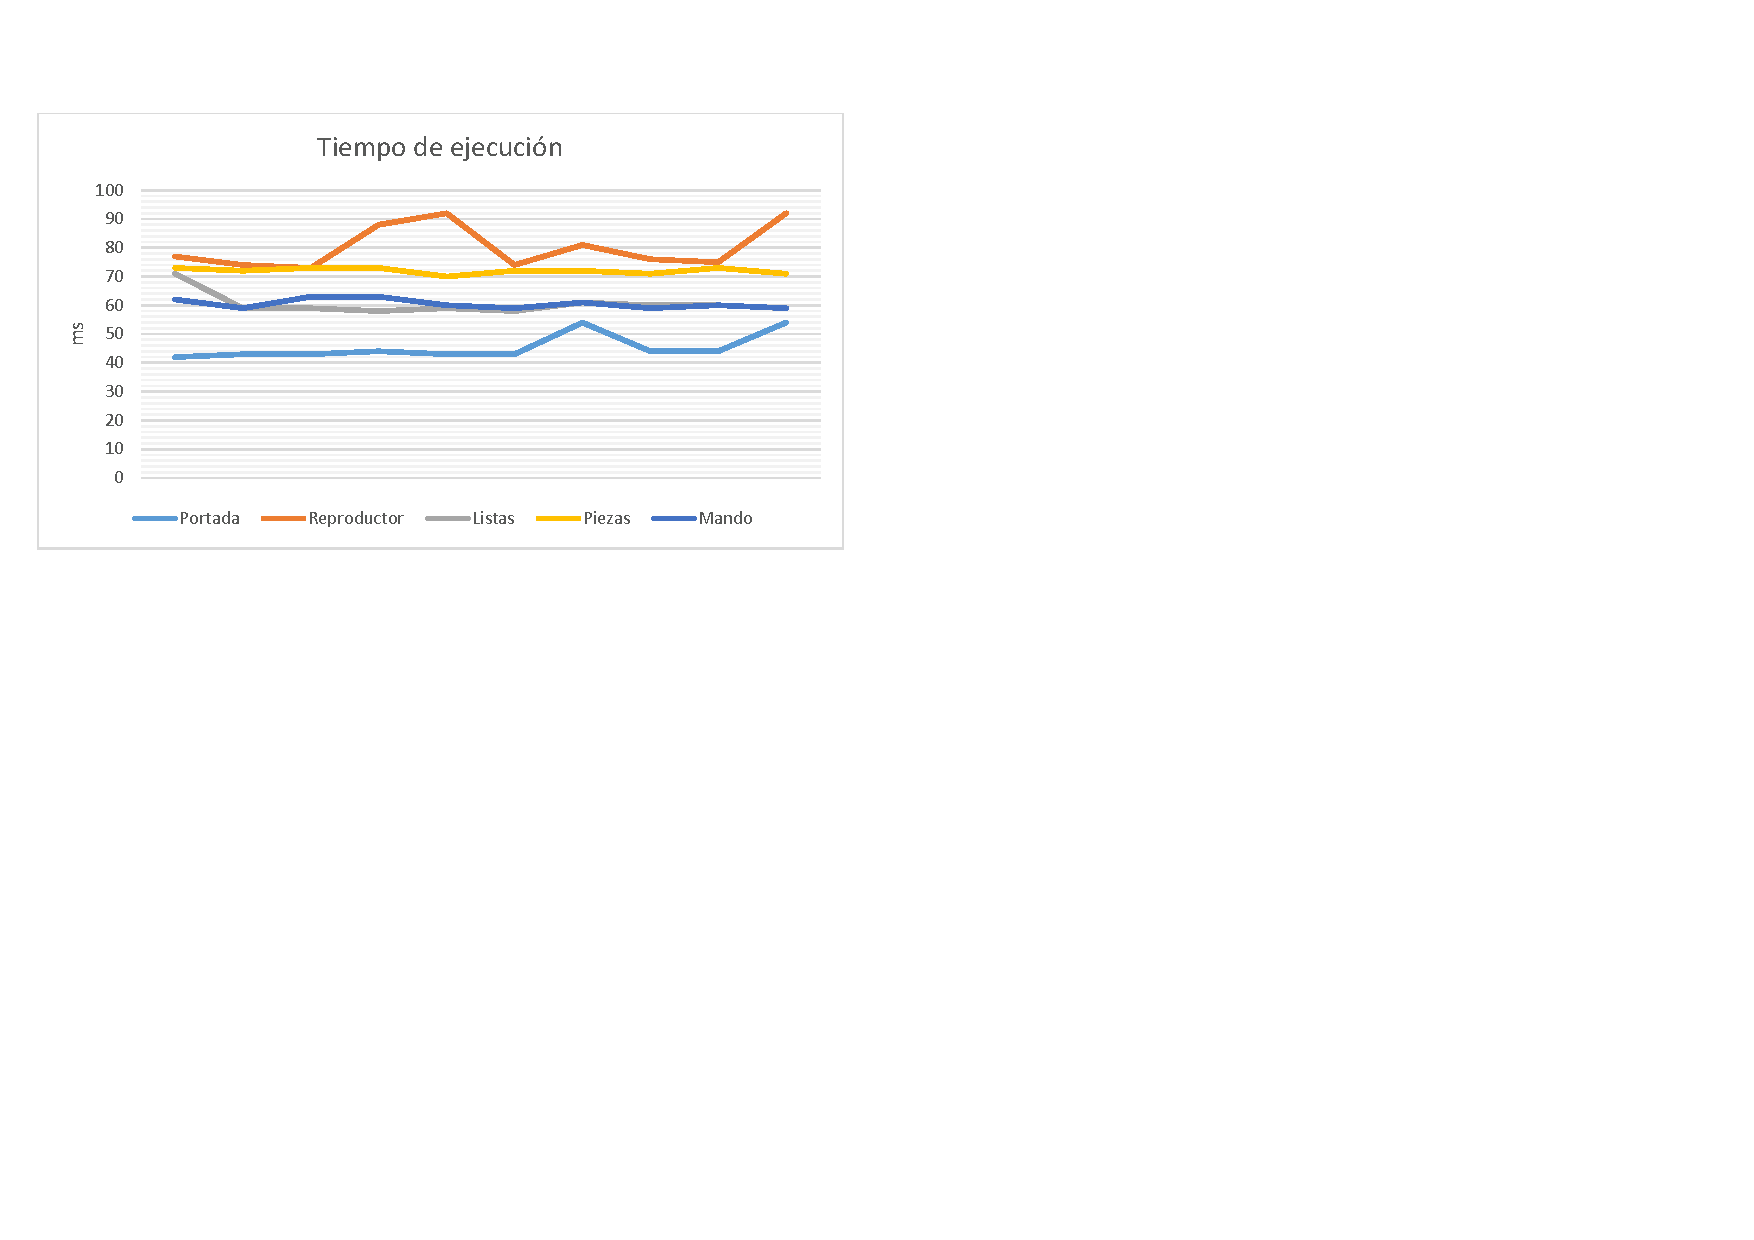
\includegraphics[width=\linewidth*3/4]{capitulo6/ejecucion_web}
		\par\end{centering}
	\smallskip
	\caption{\label{fig:ejecucion_web} Tiempo de ejecución de las vistas.}
\end{figure} 

\smallskip

Todas ellas están \textbf{por debajo de 100 \textit{ms}}. La más \textbf{rápida} es la portada, ya que no tiene que consultar información en la base de datos, mientras que el \textbf{reproductor} supera al resto, ya que tiene que comunicarse, además, con el demonio, aunque el tiempo extra es aceptable.

\subsection{Compatibilidad}

La interfaz se ha implementado en \acrshort{HTML}5 y \acrshort{CSS} 3.0. Cualquier navegador que los soporte debería funcionar sin problemas. Por nuestra parte, hemos probado la \textit{web} con las siguientes aplicaciones:

\begin{enumerate}
	\item Google Chrome 45 en Windows 8.1.
	\item Mozilla Firefox 40 en Windows 8.1.
	\item Microsoft Internt Explorer 11 en Windows 8.1.
	\item Microsoft Edge 20 en Windows 10.
	\item Firefox 40 en Ubuntu 15.04.
	\item Firefox 40 en Fedora 22.
	\item Google Chrome 45 en Mac OS Yosemite.
	\item Safari 8 en Mac OS Yosemite.
	\item Google Chrome 45 en Android 4.0.2 y 5.1.1.
\end{enumerate}

A continuación presentamos las \textbf{incidencias} que hemos encontrado:

\begin{enumerate}
	\item La página \textbf{no es compatible} con Internet Explorer, por su escaso soporte de \acrshort{CSS}.
	\item En Edge, sin embargo, funciona todo excepto ``arrastrar y soltar''.
	\item En Ubuntu tampoco funciona la función ``arrastrar y soltar'', por un \textbf{\textit{bug} en Unity} \cite{unity_bug}.
	\item Safari no soporta la \textbf{validación de formulario} (permite introducir campos en blanco), aunque sigue apareciendo el error del controlador.
	\item Safari tampoco permite \textbf{descargar} un \acrshort{MIDI} haciendo clic directamente, si no hay un reproductor compatible. En cambio, se puede hacer seleccionando ``Guardar enlace como...''
	\item No hemos podido verificar la función ``arrastrar y soltar'' en Android.
\end{enumerate}

A pesar de los problemas encontrados, exceptuando Internet Explorer, en el resto de sistemas la aplicación es totalmente \textbf{funcional y estética}. 

\subsection{Aplicaciones auxiliares}

Estas aplicaciones han servido de soporte a los bloques anteriormente descritos, de forma que podemos decir que \textbf{cumplen los requisitos}, pues de otra forma, habríamos descubierto los problemas en las pruebas anteriores.

No obstante, la \textbf{interfaz} utiliza el analizador de \acrshort{MIDI} y la aplicación de autentificación, y es interesante conocer el tiempo que emplea en usarlos.

Hemos realizado con la herramienta \code{time} una \textbf{medición superficial} del tiempo de ejecución desde consola de las siguientes órdenes:

\begin{enumerate}
	\item \code{organ status}
	\item \code{organ-midinfo --duration beethoven.mid}
	\item \code{organ-login pi}
\end{enumerate}

A continuación mostramos el resultado de \textbf{10 ejecuciones}:

\smallskip

\begin{figure}[H]
	\noindent \begin{centering}
		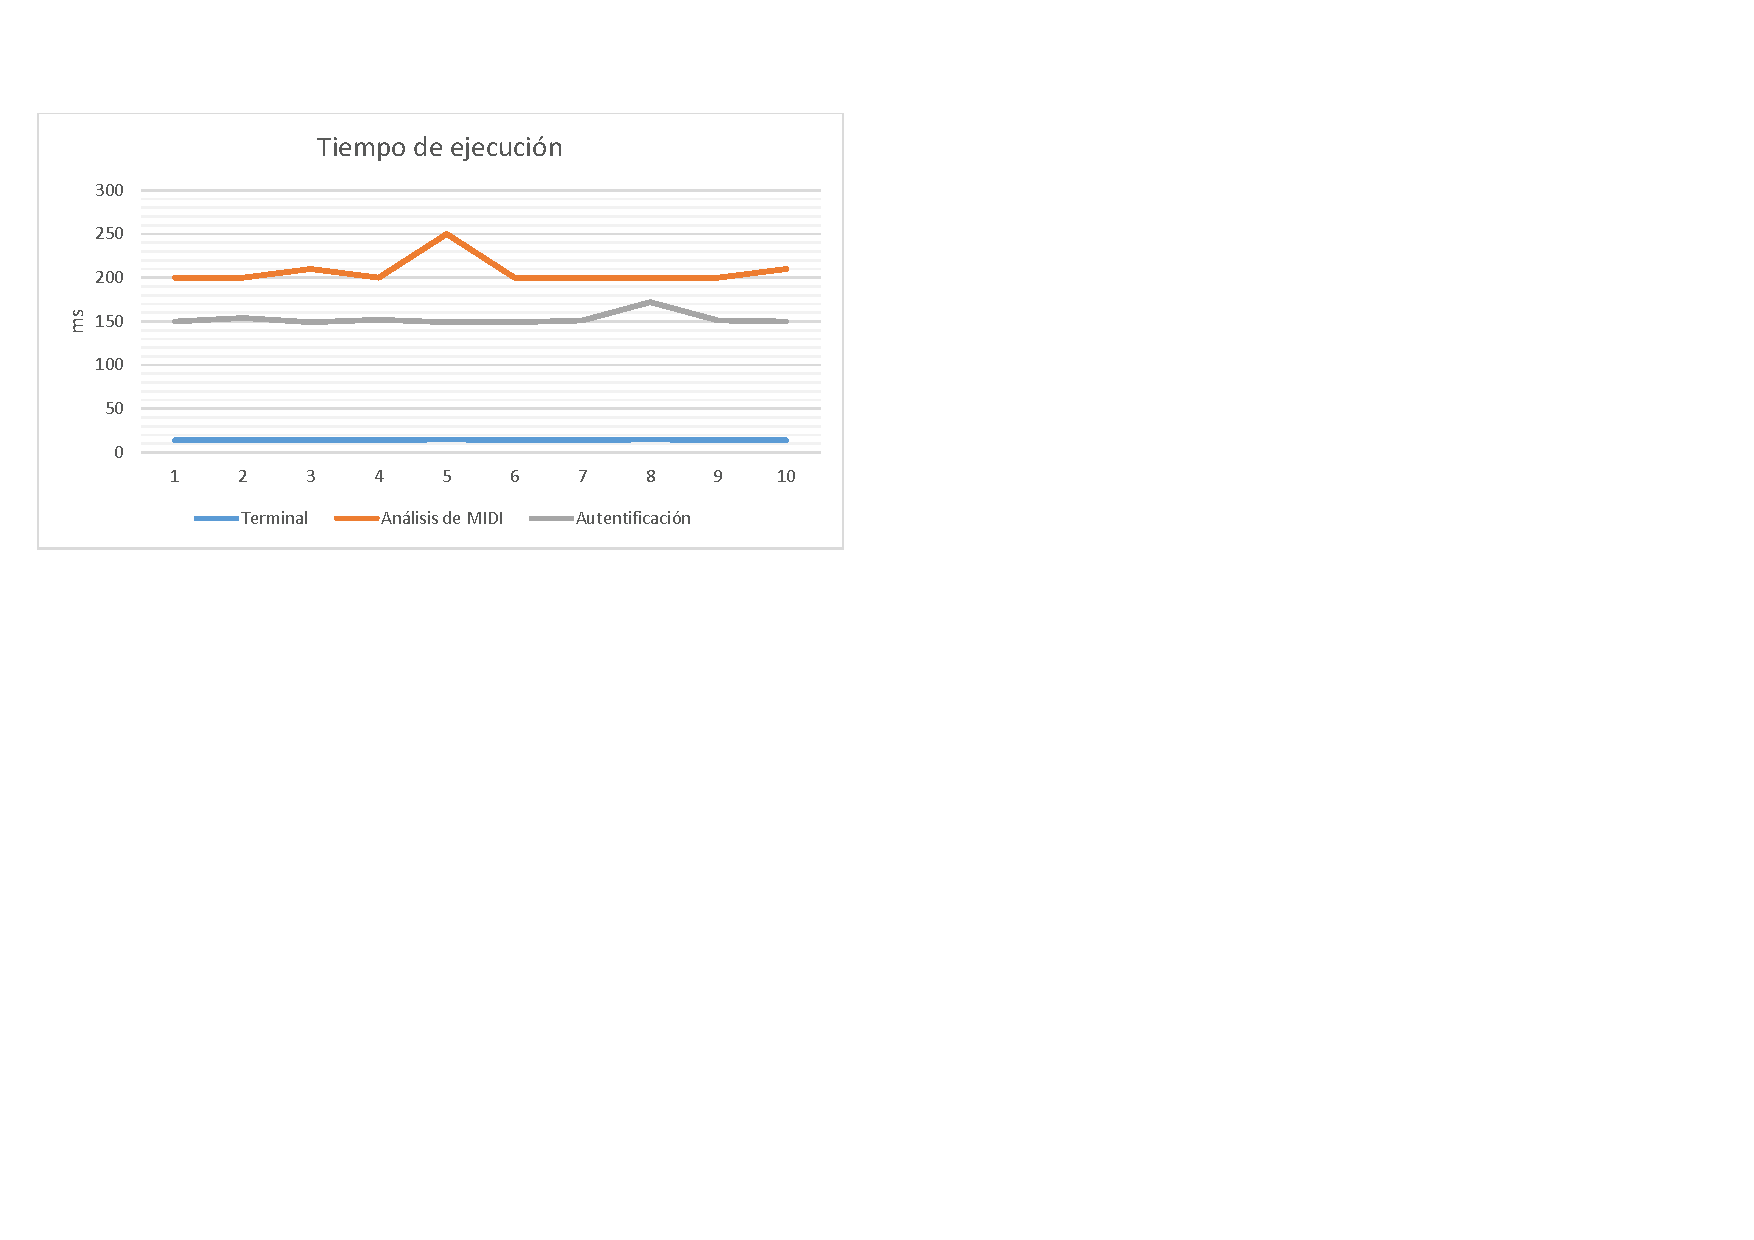
\includegraphics[width=\linewidth*3/4]{capitulo6/ejecucion}
		\par\end{centering}
	\smallskip
	\caption{\label{fig:ejecucion} Tiempo de ejecución de los programas auxiliares.}
\end{figure}

\smallskip

El resultado más sorprendente es el del \textbf{analizador}, cuya ejecución total es de 207 \textit{ms} de media, cuando la propia función de análisis solo tarda una media de 5,41 \textit{ms}.

\newpage

\section{Prueba sobre la PCB}

En último lugar, volvemos a reunirnos con Mikel Aguayo para validar nuestros \textbf{proyectos en conjunto}, tal como teníamos previsto. Actualmente solo disponemos de un \textbf{prototipo} del circuito impreso diseñado, más que suficiente para comprobar que el sistema funciona y se comporta como esperábamos.

De acuerdo a la especificación, la \acrshort{PCB} alimenta al \textit{Raspberry Pi} y se conecta, mediante unos conectores situados en la parte inferior, al banco de puertos \acrshort{GPIO} del computador.

\smallskip

\begin{figure}[H]
	\noindent \begin{centering}
		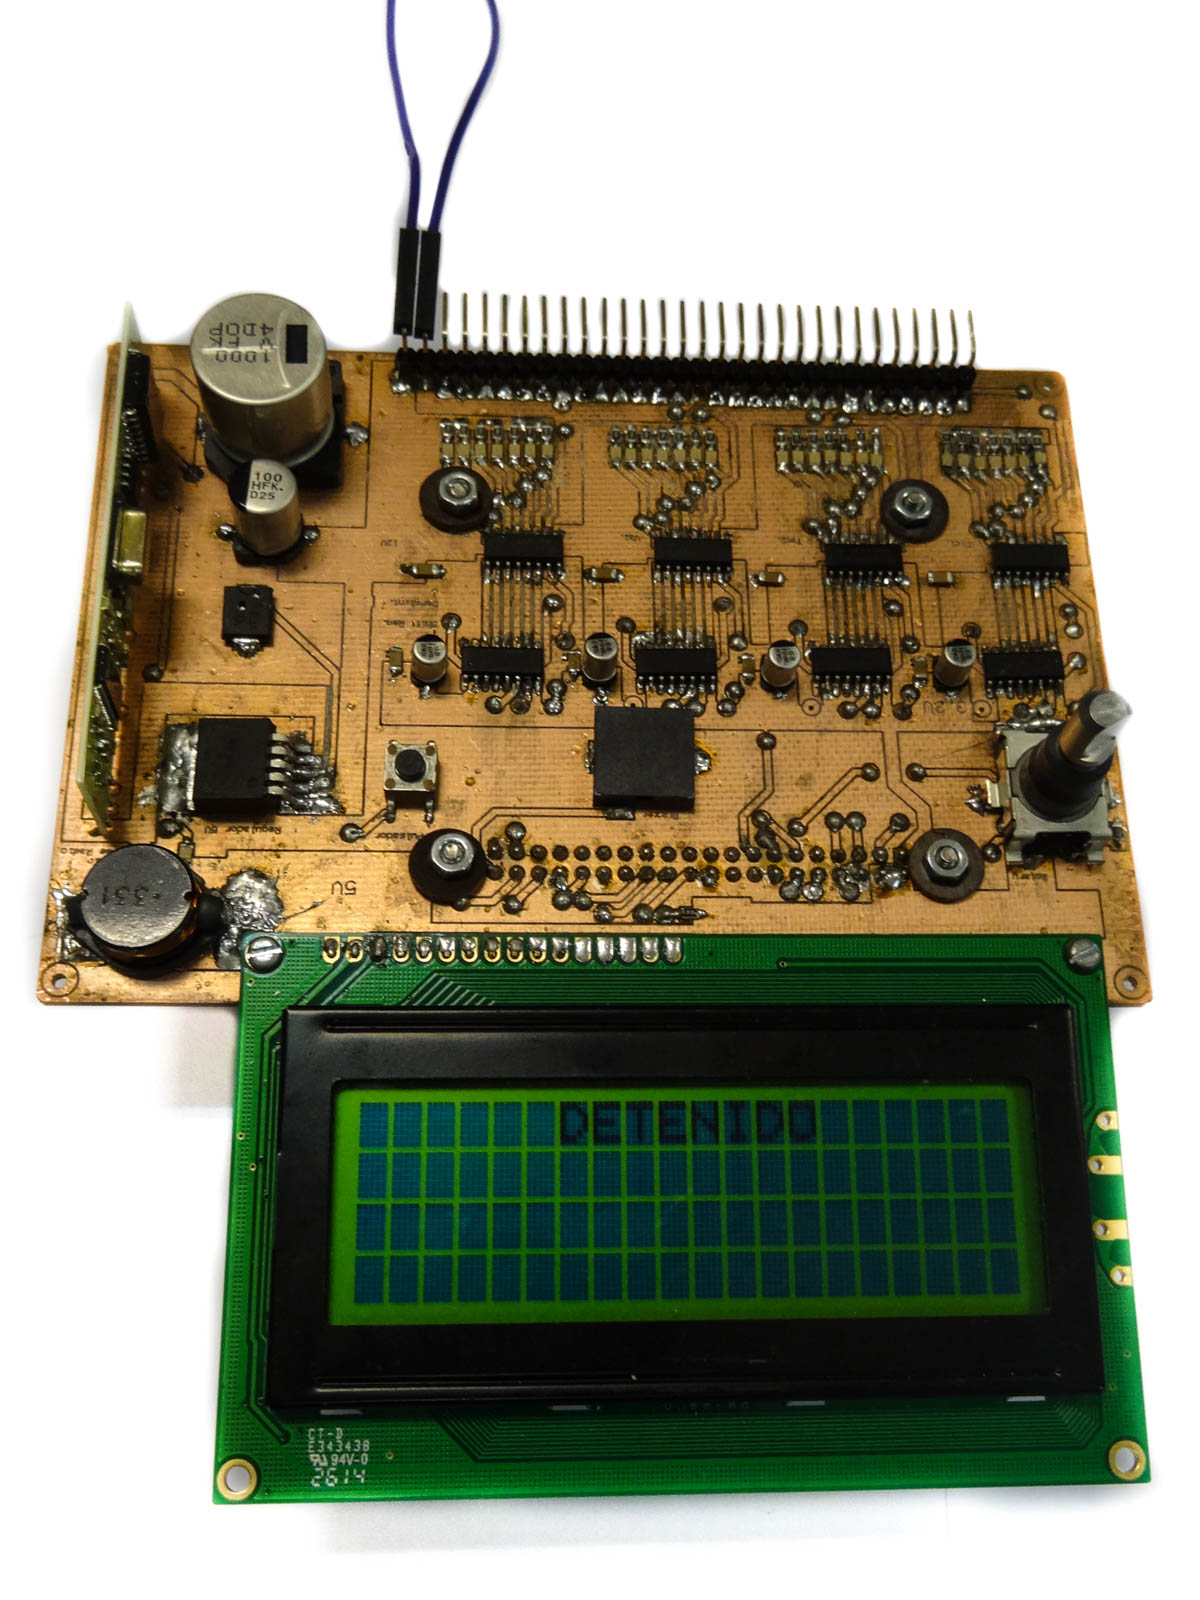
\includegraphics[width=\linewidth*3/4]{capitulo6/pcb}
		\par\end{centering}
	\smallskip
	\caption{\label{fig:pcb} Prototipo hardware.}
\end{figure} 

\smallskip

Cuando conectamos la fuente de alimentación, el \textit{Raspberry Pi} arranca automáticamente hasta que aparece ``DETENIDO'' en el \acrshort{LCD} del prototipo, que indica que la carga ha finalizado y el dispositivo está listo para funcionar.

El módulo receptor del mando responde a todos los mandos sin necesidad de \textbf{registrarlos}, ya que envía el nº de serie al \textit{software}, y éste se encarga de gestionar la pulsación.

\subsection{Entrada de datos}

Sobre la placa hemos probado dos \textbf{versiones} del \textit{software}:

\begin{enumerate}
	\item \textbf{Prototipo} en Python con una combinación fija de notas, como prueba de concepto.
	\item Implementación \textbf{final} del módulo \textit{software} de salida por \acrshort{GPIO}.
\end{enumerate}

En el prototipo establecimos un \textbf{ancho de pulso} muy grande, del orden de 1 \textit{ms}, para descartarlo de antemano de cualquier otro problema que pudiera surgir. La primera prueba fue satisfactoria como \textbf{prueba de concepto}, sin embargo, producía errores en la salida, debido a desfases producidos por el intérprete Python, pues sucedía casi determinísticamente en el 4º canal, independientemente del que escogiéramos.

Utilizamos un \textbf{osciloscopio} para realizar medidas sobre las señales que el \textit{software} envía a la \acrshort{PCB}. Aquí podemos ver el \textbf{ancho de pulso} de reloj:

\smallskip

\begin{figure}[H]
	\noindent \begin{centering}
		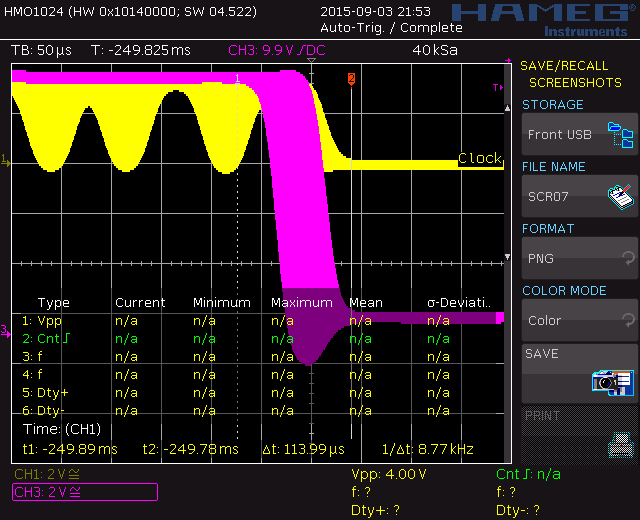
\includegraphics[width=\linewidth*2/3]{capitulo6/osc_pulso}
		\par\end{centering}
	\smallskip
	\caption{\label{fig:osc_pulso} Ancho de pulso.}
\end{figure} 

\smallskip

Tal como vemos, el lapso es de $114 \; \mu s$, que se ajusta aceptablemente a la espera requerida. 

La \textbf{segunda implementación}, ya en lenguaje C, elimina por completo este problema. Entonces ajustamos más finamente los parámetros según las especificaciones. Algunos de los \textbf{cambios} que realizamos fueron:

\begin{enumerate}
	\item Establecer el ancho de pulso del \textbf{reloj} a 100 \textit{ms}.
	\item Almacenar el nº de serie del \textbf{mando} a distancia.
\end{enumerate}

%También observamos el tiempo total en \textbf{volcar una nota}, desde que se desplaza el primer \textit{bit} hasta que se se copian los valores a la salida del registro de desplazamiento:

%\smallskip

%\begin{figure}[H]
%	\noindent \begin{centering}
%		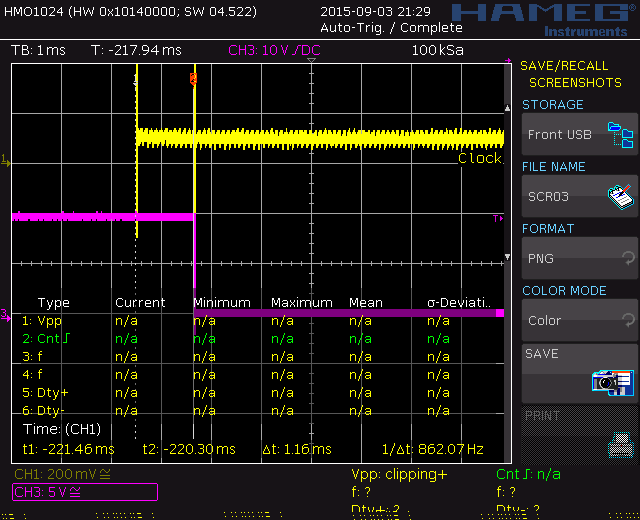
\includegraphics[width=\linewidth*2/3]{capitulo6/osc_nota}
%		\par\end{centering}
%	\smallskip
%	\caption{\label{fig:osc_nota} Tiempo de transmisión de una nota.}
%\end{figure} 

%\smallskip

%El aparato nos marca 1,16 \textit{ms}.

\subsection{Modo Ingeniería}

Éste es el nombre que hemos acuñado para el \textbf{control reducido}, que facilita un menú con cuatro funciones:

\begin{enumerate}
	\item Informar del estado del \textbf{reproductor}.
	\item Controlar el \textbf{modo Ingeniería} propiamente dicho.
	\item Activar y desactivar el \textbf{metrónomo}.
	\item \textbf{Apagar} y reiniciar el sistema.
\end{enumerate}

\smallskip

\begin{figure}[H]
	\noindent \begin{centering}
		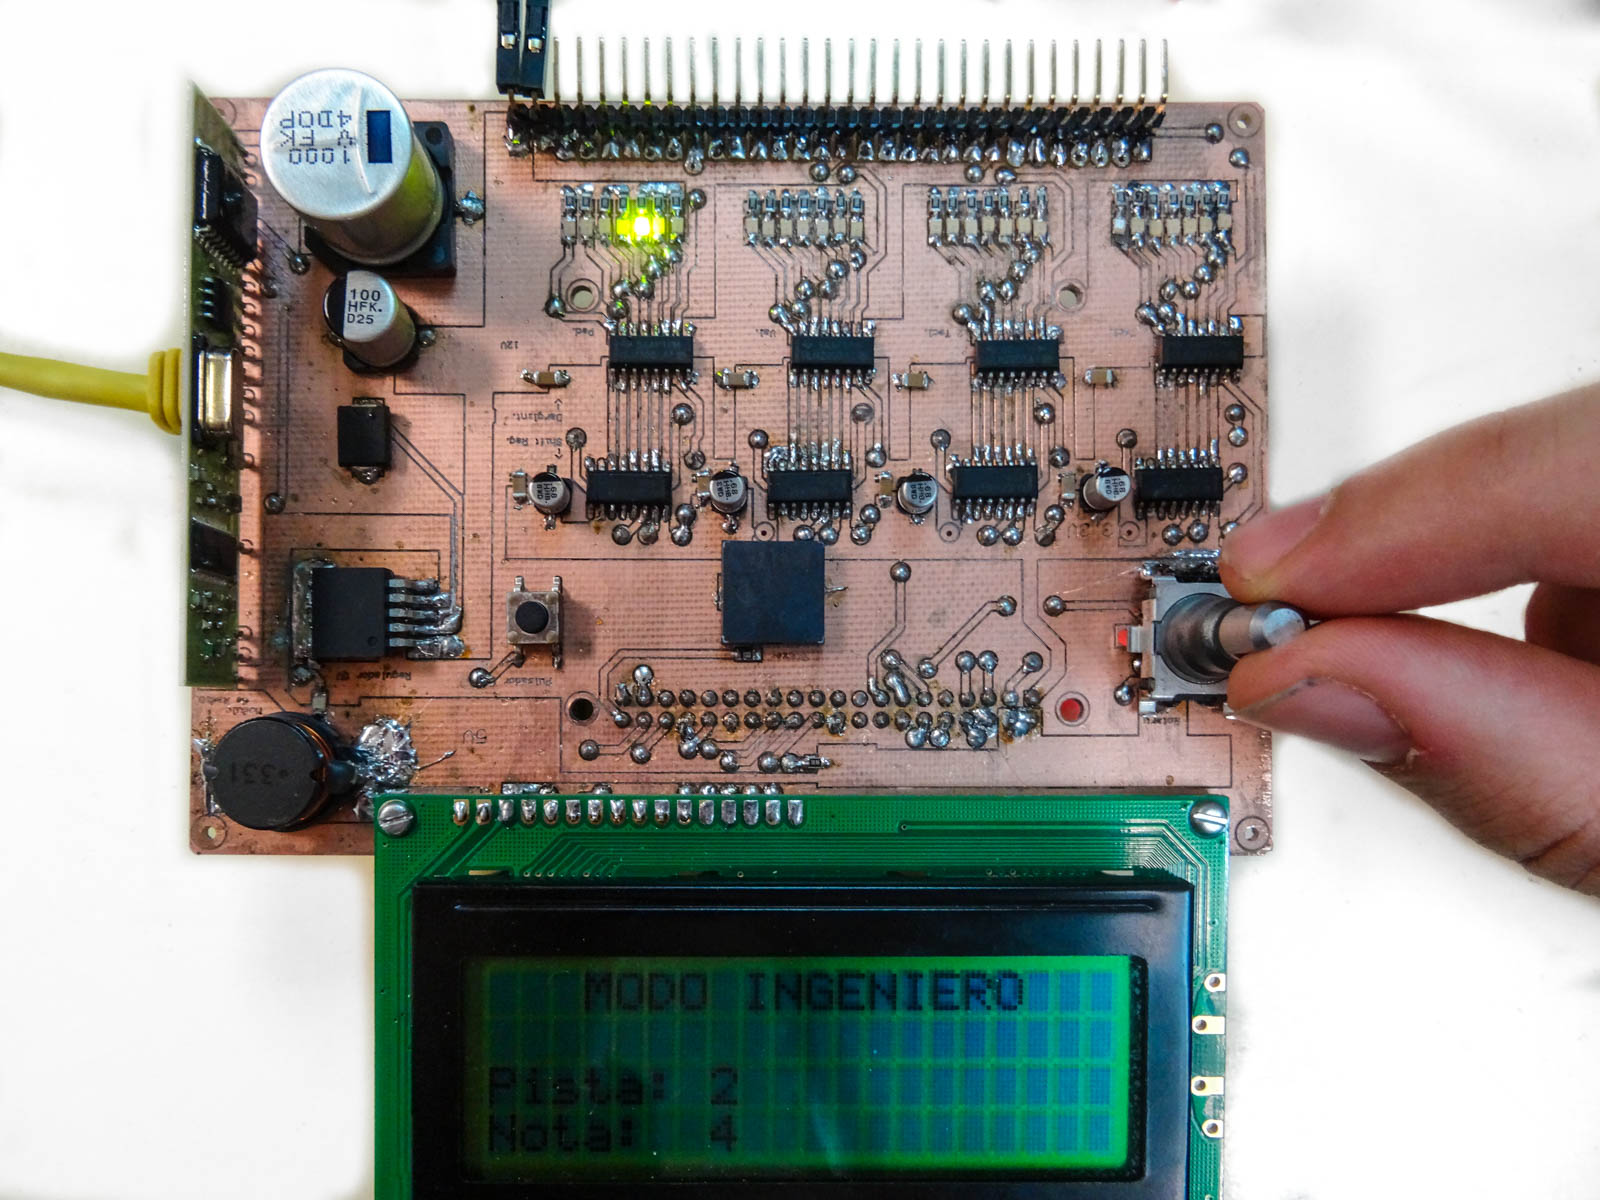
\includegraphics[width=\linewidth*3/4]{capitulo6/pcb_ingeniero}
		\par\end{centering}
	\smallskip
	\caption{\label{fig:pcb_ingeniero} PCB en modo Ingeniería.}
\end{figure} 

\smallskip

Las pruebas de validación de este módulo han sido tres:

\begin{enumerate}
	\item Comprobar que el \textit{software} recibe correctamente las señales de giro y pulsación del codificador rotatorio.
	
	\item Verificar que el menú realiza las funciones indicadas, de acuerdo a la máquina de estados diseñada en la figura \ref{fig:engineer}.
	
	\item Probar que el metrónomo funciona correctamente y que se puede apagar y reiniciar el sistema.
\end{enumerate}

Durante la prueba del control remoto pudimos detectar tres pequeños problemas:

\begin{enumerate}
	\item El \textit{software} reconocía los giros del codificador \textbf{al revés}, discrepando de la especificación de la tabla \ref{tab:info_rotary}.
	\item Se producían algunos \textbf{rebotes} en el pulsador.
	\item Apenas se escuchaba el \textbf{metrónomo}, por tener un ancho de pulso muy pequeño.
\end{enumerate}

Por tanto, se realizaron las siguientes \textbf{medidas correctoras}:

\begin{enumerate}
	\item Reajustar el sentido de giro.
	\item Aumentar la tolerancia de rebote.
	\item Regular el ancho de pulso del metrónomo para maximizar la acústica, bastante tenue.
\end{enumerate}

Aplicados estos pequeños cambios, la \acrshort{PCB} y el \textit{software} fueron capaces de comunicarse perfectamente, haciendo funcionar la reproducción de partituras tanto desde la interfaz \textit{web} como desde el mando a distancia, y manejando eficazmente el control remoto. 

Hecho todo esto, podemos dar por \textbf{completada} la fase de verificación de los objetivos propuestos en este proyecto.

\subsection{Vídeo del funcionamiento de la PCB}

\smallskip

\begin{center}
	Para reproducir este vídeo, es necesario utilizar Adobe Reader 9 o superior.
	\smallskip
	\flashmovie[engine=flv-player,width=11cm,height=6cm,auto=1,controlbar=0]{capitulo6/video_pcb.mp4}
	\smallskip
	\captionof{figure}{\label{fig:video_pcb} Vídeo del funcionamiento de la PCB.}
\end{center}

\smallskip

\newpage
\clearpage{\pagestyle{empty}\cleardoublepage}